\documentclass[10pt,twocolumn,letterpaper]{article}

\usepackage[letterpaper, top=1in, bottom=1in, left=0.75in, right=0.75in]{geometry}
\usepackage[T1]{fontenc}
\usepackage[utf8]{inputenc}
\usepackage[english]{babel}
\usepackage{lmodern}
\usepackage{microtype}

\usepackage{amsmath}
\usepackage{amssymb}
\usepackage{booktabs}
\usepackage{multirow}
\usepackage{url}
\usepackage{xurl}
\usepackage[hidelinks,breaklinks=true]{hyperref}
\usepackage{graphicx}
\usepackage{tabularx}
\usepackage{array}
\usepackage{enumitem}
\usepackage{xcolor}
\usepackage{tikz}
\usepackage{pgfplots}
\pgfplotsset{compat=1.18}
\usetikzlibrary{patterns,calc,decorations.pathreplacing}
\usepackage{draftwatermark}
\SetWatermarkText{DRAFT}
\SetWatermarkScale{1.2}
\SetWatermarkColor[gray]{0.92}
\setlength{\parskip}{0pt}
\setlength{\parsep}{0pt}
\setlength{\columnsep}{0.25in}

\title{\Large\textbf{Before the Runway Expires: A Compliance Posture Framework\\for Early Engagement in the Web PKI}\\[0.5em]
\normalsize\textit{Working Draft --- Not for citation or distribution}}

\author{
Research\\
\textit{Systematic Reasoning, Inc.}\\
\texttt{info@systematicreasoning.com}
}

\date{}

\begin{document}

\maketitle

\begin{abstract}
The median time from first Bugzilla compliance signal to CA distrust across graduated-pathway
removals is 1,185 days. This paper asks not whether that evidence was eventually sufficient to
justify action---it was---but whether it was readable earlier, and whether reading it earlier
could have changed what happened. Prior work in this series established that auditors detect
only 29.2\% of in-period incidents~\cite{p1} and that root program Bugzilla coverage has
fallen below 20\%~\cite{p2}. Neither paper addresses whether detected incidents are fixed.

We propose the \textit{Compliance Posture Framework} (CPF), combining two independently
computed observables from public Bugzilla data: the \textit{Accountability Loop Score} (ALS),
measuring structural non-remediation through chronic incident class recurrence, and the
\textit{Incident Response Quality} (IRQ) score, measuring behavioral posture via LLM-assisted
classification of 1,616 compliance thread arcs. Together they produce an \textit{Engagement
Priority Score} (EPS, 0--100) that addresses three operational questions from the same
public data: for root programs, which CAs warrant proactive engagement before the record
forces action; for CAs, where are the accountability loops in my own compliance record
not closing; and for auditors, which failure modes in the public record should direct
fieldwork scope and calibrate skepticism about management representations.

The framework is validated against the 16-event distrust taxonomy. All three
graduated-pathway CAs with sufficient data flag correctly. Crucially, Entrust---the most
recent and largest distrust case---was flagged by the ALS as early as 2019, five years
before its 2024--2025 distrust proceedings, when only 6 of 35 active CAs (17\%) carried
the same signal. The temporal signal was available. The engagement question is whether it
was used.

Among the current trusted population of 51 active CAs, 76\% have at least one chronic
incident class, 41\% have three or more, and 15 (29\%) match the full graduated-pathway
distrust profile. Independently, LLM-assisted classification of 1,616 Bugzilla thread
arcs reveals that distrusted CAs resolve incidents cleanly at half the rate of active
CAs (47\% vs.\ 79.9\% healthy arcs) and experience accountability pressure at nearly
double the rate (29\% vs.\ 17\%). Escalating-arc threads---where the CA contests
requirements rather than failing to meet them---are 8.8$\times$ more prevalent in
distrusted records ($p < 10^{-12}$, OR~$=9.6$, 95\%~CI~4.6--20.0). The framework does not predict distrust.
It maps where the accountability loop is structurally open and where behavioral posture
signals that the loop will not close without external pressure. The same signals that
enable root program engagement prioritization allow CAs to identify structural
non-remediation in their own record before it becomes a governance conversation.
\end{abstract}

\section{Introduction}
\label{sec:intro}

Root programs remove certificate authorities. Since 2011, sixteen CA organizations have
been distrusted by at least one major root program. The removal decisions were not
arbitrary. Each followed years of documented evidence that something was structurally
wrong---compliance failures recurring across annual audit cycles, root program pressure
that produced reports without fixing root causes, and behavioral posture that experienced
reviewers came to recognize as irremediable. The median time from first Bugzilla signal to
distrust across graduated-pathway removals is 1,185 days.

That figure is not a measure of the evidence's eventual strength. It is a measure of how
long a governance process operating on voluntary engagement and annual audit cycles takes
to assemble enough of it. Entrust accumulated 71 Bugzilla incidents over eight years
before its 2024--2025 distrust proceedings. The question is not whether the eventual
record was sufficient. It was. The question is whether the structural and behavioral
signals present in year three were readable as a flag for early engagement---and whether
acting on them at year three rather than year eight would have changed the outcome.

Prior work in this series has documented two other aspects of the detection problem.
The first paper~\cite{p1} established that auditors detect only 29.2\% of in-period
Bugzilla incidents in their letters---a structural ceiling on the formal audit channel's
contribution. The second paper~\cite{p2} established that root program Bugzilla coverage
has declined below 20\% for both Chrome and Mozilla, while CA self-monitoring has grown
to 46.1\% of filings in 2025. Both papers describe detection failures. Neither addresses
whether detected incidents are fixed.

This paper argues that the more consequential question for the governance system is
remediation, not detection. A CA that finds its own problems and fixes the structural
conditions producing them is exhibiting the behavior the accountability system was designed
to produce. The same CA, if the same failure class recurs in subsequent calendar years,
is exhibiting failed remediation regardless of who found the problem. The structural
signature of this failure is observable in public Bugzilla data as \textit{chronic class
recurrence}---the same incident whiteboard tag appearing across three or more distinct
years for the same CA.

\textbf{Contributions.}
\begin{itemize}[noitemsep,topsep=2pt]
\item \textit{Accountability Loop Score (ALS).} A fully specified composite observable
  from public Bugzilla data and CCADB audit records, measuring detection quality,
  structural non-remediation via chronic class recurrence with ecosystem spike correction,
  incident acceleration, and governance incident share. Formally specified in
  Section~\ref{sec:als} with complete notation.
\item \textit{Temporal validation.} Retrospective computation of ALS at each calendar
  year for the three graduated-pathway distrusted CAs. Entrust was flagged in 2019---five
  years before distrust---when the framework's alarm rate across the active population
  was 17\% (Section~\ref{sec:temporal}).
\item \textit{Incident Response Quality (IRQ).} LLM-assisted classification of 1,616
  Bugzilla thread arcs into five behavioral categories. Distrusted CAs resolve incidents
  cleanly at half the rate of active CAs (47\% vs.\ 79.9\% healthy arcs), experience
  accountability pressure at nearly double the rate, and show escalating-arc prevalence
  8.8$\times$ higher ($p < 10^{-12}$, OR~9.6). Pattern connection response---a
  classification-independent signal measuring whether CAs address systemic framing when
  offered---provides an additional behavioral observable immune to LLM classifier
  sensitivity (Section~\ref{sec:irq}).
\item \textit{Engagement Priority Score (EPS).} A unified 0--100 indicator combining ALS
  and IRQ: EPS answers ``should I look closer?''; the component scores answer ``why'' and
  ``what kind of engagement.'' All three graduated-pathway CAs rank in the top 16\% by EPS
  across 63 CAs (Section~\ref{sec:eps}).
\item \textit{Cross-thread pattern synthesis.} A third pipeline pass using a larger
  language model synthesizes each CA's complete commitment and incident history to
  identify recurring \textit{architectural} patterns --- cases where later incidents
  share root cause with prior commitments even when the specific manifestation differs.
  Validated on DigiCert: the ``fail-open under degraded conditions'' pattern links a
  2017 CAA timeout incident to a 2026 MPIC network disruption, revealing the same
  design weakness (validation defaulting to permit under failure) persisting across
  9 years and multiple surface-level incident classes.
\item \textit{Multi-stakeholder interpretation.} The same signals support
  distinct readings for three audiences. Root programs use EPS for engagement
  prioritization. CAs apply the signals to their own record to identify unresolved
  failure modes, monitoring gaps, and incident response quality deficits before they
  become governance conversations. Auditors use the chronic class inventory, self-report
  rate, and arc distribution as pre-engagement scoping inputs that direct fieldwork at
  the failure modes the public record already shows are unresolved---addressing the
  detection gap documented in prior work~\cite{p1} from the audit preparation side
  (Section~\ref{sec:discussion}).
\item \textit{Ecosystem spike correction and comparable cases.} Identification and
  application of a floor-based ecosystem factor ($f_\text{eco} \geq 0.85$) that
  distinguishes independent chronic recurrence from ecosystem-wide enforcement sweeps,
  and comparable-case matching between current active CAs and historical distrust
  profiles (Section~\ref{sec:population}).
\end{itemize}

\section{Background}
\label{sec:background}

\subsection{The distrust record}

The WebPKI Observatory maintains a curated taxonomy of all 16 CA distrust events from
2011 through 2025, classifying each by compliance posture, distrust pathway, root cause,
and response quality. Seven removals followed a \textit{graduated} pathway---an extended
period of Bugzilla accumulation before action. Four followed an \textit{immediate} pathway
driven by a single catastrophic event (infrastructure compromise, intelligence affiliation
disclosure). Four were \textit{triggered} by external discovery of a specific violation.
One was \textit{negotiated}.

The graduated pathway is the one this framework targets. Immediate-pathway cases (DigiNotar,
WoSign) involved deliberate concealment or catastrophic single failures generating little
prior Bugzilla record. The ALS correctly assigns these cases low scores---not as a
limitation but as the correct output: the accountability mechanism that generates our
signal (the public Bugzilla thread) was bypassed or nonexistent before these cases
triggered enforcement. A framework that flags Camerfirma and not DigiNotar is correctly
describing what the public record contains and what it does not.

Of the seven graduated-pathway cases, four have Bugzilla records meeting the minimum
confidence threshold of ten bugs. Certinomis (18 bugs, 2016--2020), Camerfirma (46 bugs,
2017--2021), and Entrust (71 bugs, 2017--2025) constitute the primary validation set.
e-Tugra (14 bugs, 2021--2023), while formally classified as triggered, exhibits
gradual-accumulation properties and is analyzed separately. The three remaining graduated
cases---PROCERT, TurkTrust, Visa---predate the dense Bugzilla era and have insufficient
records for ALS scoring.

\subsection{The three-actor structure}

The accountability loop involves three actors. The \textit{CA} discovers and files
incidents; its self-report rate reflects monitoring investment and disclosure willingness.
The \textit{auditor} produces the annual assurance letter; prior work~\cite{p1} established
that auditors mention only 29.2\% of in-period incidents, providing limited formal
verification. The \textit{root program} reads both channels and decides whether to engage.

The CA selects and compensates the auditor, creating known incentives for the CA to
prefer auditors whose engagement does not deeply probe the incident record. And root
program Bugzilla coverage has declined below 20\% for both Chrome and Mozilla~\cite{p2}.
These conditions make high self-report rate and formal audit compliance necessary but
insufficient evidence of a healthy accountability loop. The Entrust case makes this
concrete: 84\% self-report rate, four chronic incident classes across eight years, eventual
distrust in 2024--2025. Entrust found its problems. It did not fix the structural
conditions producing them. An accountability framework that rewards detection without
measuring remediation will systematically miss this failure mode.

\subsection{Why incident volume is insufficient}

Raw incident count is a poor posture signal for a structural reason: it correlates with
issuance volume and compliance team activity, not compliance posture. DigiCert has 171
Bugzilla incidents; it has not been distrusted. Let's Encrypt has 38; it is broadly
regarded as a compliance exemplar. A large CA with active self-monitoring and prompt
remediation accumulates more incidents than a small CA that monitors nothing---and the
former is exhibiting better accountability behavior.

The signal that escapes this confound is class recurrence. A CA that files an
\texttt{ov-misissuance} incident in 2019, performs credible root cause analysis, and never
files another has closed the accountability loop. A CA that files \texttt{ov-misissuance}
incidents in 2019, 2020, 2021, 2022, and 2023 has not---regardless of whether any
individual incident was self-reported. The multi-year recurrence of the same tag is direct
evidence that root-cause remediation either did not occur or did not address the systemic
condition.

\subsection{Related work}

Durumeric et al.~\cite{durumeric2013} established the baseline ecosystem measurement
methodology. Liu et al.~\cite{liu2015} measured revocation end-to-end. Sun et
al.~\cite{sun2024} revisited CT monitoring infrastructure. Amann et al.~\cite{amann2017}
measured the ecosystem's response to the Symantec distrust, establishing that the
gradual-then-sudden pattern is observable across the distrust record and that recovery
after large-CA removal is measurable and slow. This paper is the first to measure the
compliance posture signals that precede the ``suddenly'' phase using the public Bugzilla
record as the primary instrument, and the first to compute those signals retrospectively
across calendar years to ask when the signal became readable.

\section{The Accountability Loop Score}
\label{sec:als}

\subsection{Formal specification}

Let $B_c$ denote the set of Bugzilla compliance bugs attributed to CA $c$, after
batch collapse (same-day filings of three or more bugs with identical tag sets are
collapsed to one representative event, correcting for ETSI audit-finding batches).
Let $n = |B_c|$ with confidence weight $\text{conf} = \min(n/15, 1)$.

For each bug $b \in B_c$, let $\text{year}(b)$, $\text{quarter}(b)$, and
$\text{tags}_c(b)$ denote the filing year, calendar quarter, and whiteboard tags
after excluding \texttt{audit-finding} and \texttt{uncategorized} (see
Section~\ref{sec:exclusions}). Define:

\begin{align}
\text{tag\_years}[t] &= \{\text{year}(b) : b \in B_c,\; t \in \text{tags}_c(b)\} \notag \\
\text{tag\_solo}[t] &= \{\text{year}(b) : b \in B_c,\; t \in \text{tags}_c(b), \notag \\
   &\quad\quad\quad \sigma(t, \text{quarter}(b)) < 5\} \notag
\end{align}

where $\sigma(t, q)$ is the count of distinct CAs filing tag $t$ in quarter $q$
(from the ecosystem spike index, Section~\ref{sec:ecosystem}).

\textbf{Chronic class detection.}
\[
\mathcal{C} = \{t : |\text{tag\_years}[t]| \geq 3\}, \quad n_c = |\mathcal{C}|
\]

\textbf{Ecosystem correction.}
\[
\mathcal{C}_{\text{solo}} = \{t \in \mathcal{C} : |\text{tag\_solo}[t]| \geq 3\}
\]
\[
r_{\text{solo}} = |\mathcal{C}_{\text{solo}}| / n_c \quad (0 \text{ if } n_c = 0)
\]
\[
f_{\text{eco}} = 0.85 + 0.15 \cdot r_{\text{solo}}
\]

\textbf{Scalar signals.} $r_{\text{self}}$ = fraction of bugs filed by CA staff
(email domain matched against CCADB CA owner records). $g$ = fraction of bugs
tagged with governance failure tags (\texttt{policy-failure}, \texttt{disclosure-failure}).
Incident rate $\rho = n / |\mathcal{Y}|$ where $\mathcal{Y}$ is the set of active
years. Acceleration $\alpha$ compares per-year incident rate in the recent half of
$\mathcal{Y}$ to the early half. Chronic span average
$\bar{s} = \frac{1}{n_c}\sum_{t \in \mathcal{C}} |\text{tag\_years}[t]|$.

\textbf{Mode A} (detection failure and deterioration):
\[
A = (1 - r_{\text{self}}) \cdot \text{conf} \cdot 30 + \max(0, \ln\!\max(\alpha, 0.5)) \cdot \min\!\left(\tfrac{n}{10}, 1\right) \cdot 20 + g \cdot 15
\]

\textbf{Mode B} (structural accumulation):
\begin{align}
B_1 &= \min\!\left(\tfrac{n_c - n_{\text{closed}}}{5}, 1\right) \cdot f_{\text{eco}} \cdot \bar{w}_k \cdot f_{\text{bp}} \notag \\
B_2 &= \min\!\left(\tfrac{\ln\!\max(\rho, 1)}{\ln 10}, 1\right) \notag \\
B_3 &= \min\!\left(\tfrac{\bar{s}}{7}, 1\right) \notag \\
B   &= 35 B_1 + 20 B_2 + 10 B_3 + 10 g \notag
\end{align}

where $n_{\text{closed}}$ is the number of chronic classes with a substantive
commitment (grade A, B, or C) where the last occurrence was 3 or more years
ago---evidence the loop closed; $\bar{w}_k$ is the average knowledge weight:
\[
w_k(t) = 1 + 0.5 \cdot \min\!\left(\tfrac{|\text{prior\_cas}(t,y_1)|}{20}, 1\right)
              \cdot \min\!\left(\tfrac{\text{eco\_age}(t,y_1)}{4}, 1\right)
\]
where $\text{prior\_cas}(t, y_1)$ is the number of distinct CAs that filed tag $t$
before the CA's first occurrence year $y_1$, and $\text{eco\_age}(t, y_1)$ is the
years since $t$ first appeared in the corpus ($w_k$ ranges from 1.0 to 1.5);
and $f_{\text{bp}} = \min(1 + 0.1 \cdot n_{\text{bp}},\, 1.3)$ is the broken-promise
factor, $n_{\text{bp}}$ being the number of governance-class chronic recurrences
within two years of a substantive commitment on that class.

\textbf{Final score:}
\[
\text{ALS} = \max(A, B) + \max(0, \ln\!\max(\alpha, 1)) \cdot 8 \cdot \min\!\left(\tfrac{n}{10}, 1\right)
\]

Both the deterioration signal in Mode~A and the acceleration boost are gated by
$\min(n/10, 1)$. Acceleration ratios computed across fewer than ten bugs are
noise---comparing one or two early incidents against four or five recent ones
produces large ratios that do not reflect genuine trend. The gating ensures
acceleration contributes meaningfully only when the corpus is large enough for
the comparison to be credible.

Mode A fires on operational blindness combined with deterioration (the Certinomis
profile: low self-report rate plus worsening acceleration). Mode B fires on structural
accumulation of chronic failure classes at density (the Entrust and Camerfirma
profile). The acceleration boost $\max(0, \ln\alpha)\cdot 8$ applies in both
modes when the incident rate is worsening, reflecting that a CA whose record is
getting worse faster warrants additional urgency regardless of which failure mode
is dominant.

\subsection{Mode crossover}

Mode A dominates when $(1-r_{\text{self}}) \cdot \text{conf} \cdot 30 > B$. For a CA
with zero chronic classes, $B_1 = 0$, so Mode B contributes only density and governance
signals. A CA with 14\% self-report rate contributes $0.86 \cdot 30 = 25.8$ to
Mode A from detection failure alone, typically sufficient to dominate a low-chronic
Mode B reading. This is precisely the Certinomis profile. Conversely, for Entrust with
84\% self-report rate, the detection failure contribution falls to $0.16 \cdot 30 = 4.8$,
and Mode B's chronic accumulation signal dominates. The dual-mode structure ensures that
both failure profiles---detection blindness and structural non-remediation---produce
elevated scores, while a CA performing well on both dimensions scores low on both.

\subsection{Ecosystem spike correction}
\label{sec:ecosystem}

Chronic class recurrence is designed to measure per-CA remediation failure. The
Bugzilla corpus contains identifiable periods where the same incident class appeared
simultaneously across many CAs, driven by ecosystem-wide enforcement---notably
2017-Q3 (21 CAs filed \texttt{ov-misissuance} simultaneously in Mozilla's batch
enforcement campaign) and 2019-Q1 (28 CAs under CA/B Forum Ballot SC14/SC17).

A CA filing \texttt{ov-misissuance} in 2017-Q3 alongside 20 others might seem like
a different event from one filing independently. But a CA that repeatedly fails the
same compliance class is responsible for that failure regardless of what peers were
doing at the time. ``Everyone else was also failing'' is not a mitigating factor---if
anything, a CA whose same failure class recurs across 2021, 2023, and 2024 while
peers have corrected it is exhibiting \textit{worse} remediation behavior, not
comparable behavior. Nine incidents over three years with repeating patterns is a
significant structural signal regardless of ecosystem context.

The framework therefore applies only a modest floor discount rather than a full
ecosystem correction. When a CA's chronic class years coincide entirely with
ecosystem-wide sweep quarters, the B1 scoring weight is discounted by at most 15\%
(factor $f_\text{eco} = 0.85$); when recurrence is independent of sweeps, no
discount applies ($f_\text{eco} = 1.00$). The spike index covers tag-quarter
combinations where $\geq$10 CAs filed simultaneously---a threshold that isolates
genuine enforcement waves while leaving routine background activity undiscounted.

All three graduated-pathway CAs flag at or above threshold~48 under this
formulation.

\textbf{Ecosystem knowledge weight.} The spike index is also used to compute a
\textit{knowledge weight} for each chronic class. A CA filing a failure class that
had already been documented across many other CAs---with root cause analyses published,
CA/B Forum ballots passed, and remediation expectations established---had full industry
notice. Filing the same class five years later is not the same failure as being the
first CA to encounter it.

For each chronic class tag $t$ and the year $y_1$ of the CA's first occurrence:
\[
w_k(t) = 1 + 0.5 \cdot \min\!\left(\frac{|\text{prior\_cas}(t, y_1)|}{20}, 1\right)
              \cdot \min\!\left(\frac{\text{eco\_age}(t, y_1)}{4}, 1\right)
\]
where $\text{prior\_cas}(t, y_1)$ is the number of distinct other CAs that filed tag
$t$ before year $y_1$, and $\text{eco\_age}(t, y_1)$ is the number of years since $t$
first appeared in the corpus. The weight ranges from 1.0 (genuinely novel failure class,
no prior ecosystem record) to 1.5 (well-documented class with 20+ prior CAs and 4+
years of industry precedent). The average weight $\bar{w}_k$ across a CA's chronic
classes multiplies the $B_1$ term.

\textbf{Cross-thread pattern synthesis.} The per-thread IRQ pass operates
on individual Bugzilla threads in isolation; it cannot identify when a 2026 incident
is the same architectural weakness as a 2017 commitment. A third pipeline pass using
a larger language model addresses this. The input is the CA's full commitment and
incident history (commitment text, incident summaries, RCA depth, arc classification)
across all scored threads---typically 10,000--35,000 tokens per large CA. The model
is asked to identify recurring architectural patterns: cases where later incidents
suggest prior commitments addressed the specific symptom but not the underlying root
cause, regardless of which surface-level compliance class the incident falls under.

The key instruction is to reason about root cause, not tag class. ``CAA timeout treated
as pass'' (2017) and ``CAA fails open during network disruption'' (2026) share root
cause (validation defaulting to permit under failure) even though the specific
triggering mechanism differs. No tag filter or commitment grade filter is applied:
the model reads across the full history.

Output is a structured list of patterns per CA, each with: a pattern name, a one-sentence
root cause description, the prior bugs where commitments were made on this root cause,
the later bugs where it resurfaced, confidence level, and a brief evidence summary.
Validated on DigiCert: nine patterns identified including ``fail-open under degraded
conditions,'' ``manual validation input bypassing automated controls,'' and ``timely
incident disclosure failures.'' The synthesis notes for DigiCert characterize the
CA as showing ``systematic gaps in generalizing root causes---architectural fixes
tend to address the specific mechanism rather than the underlying control philosophy.''
This cross-thread output is available per CA in the Observatory and is the primary
signal for the CA self-assessment and auditor scoping use cases.

\textbf{Commitment amplification and closed-loop credit.} The IRQ pipeline grades each
CA commitment on a scale of A through F. A grade-A commitment is one that was made
clearly, scoped to the failure class, and kept---verified by the absence of subsequent
recurrence or an explicit root program confirmation.

A chronic class with a grade-A commitment and no recurrence in subsequent years is
evidence that the accountability loop closed: the CA identified the root cause, committed
to fix it, and fixed it. These classes are subtracted from the effective chronic class
count $n_c - n_{\text{closed}}$ in the $B_1$ term, giving credit for demonstrated
remediation.

A governance-class chronic failure (\texttt{policy-failure} or
\texttt{disclosure-failure}) that recurs within two years of a grade-A commitment is
a documented broken promise: the CA told the root program exactly what it was going
to do, received credit for the commitment, and then the same systemic failure
reappeared. The broken-promise factor $f_{\text{bp}}$ applies a modest amplifier
(10\% per broken class, capped at 1.3$\times$). Operational tags are excluded from
broken-promise detection because they cover many specific certificate variants---a
commitment on one specific issuance error does not make every subsequent instance of
the same tag class the same unfixed issue.

\subsection{Exclusions from chronic detection}
\label{sec:exclusions}

Two whiteboard tags are excluded from chronic class detection.
\texttt{uncategorized} is a tagging artifact. \texttt{audit-finding} reflects
ETSI framework reporting practice: ETSI auditors file one bug per finding while
WebTrust auditors may consolidate, creating systematic ETSI overpenalization
unrelated to remediation behavior if included. Batch collapse (Section~\ref{sec:als})
addresses related multi-filing artifacts at the same-day level.

\section{Test Vector Validation}
\label{sec:testvectors}

\subsection{Threshold calibration}

The ALS threshold of 48 was calibrated as follows. The minimum score among the three
graduated-pathway CAs with sufficient data is 49.8 (Certinomis). The maximum score among CAs with zero chronic classes and self-report rates
above 60\%---the strongest candidates for a clean profile---is 44.3. The threshold of 48
sits between these, providing a 1.8-point buffer below the lowest graduated-pathway CA (Certinomis, 49.8)
and a 3.3-point buffer above the healthiest non-chronic CA.

This calibration uses the test set to set the decision boundary. For a predictive
classifier, that would be inadmissible. The framework is not a classifier: it produces
an engagement prioritization signal. The operational interpretation of ALS~$\geq 48$ is
that a CA at this threshold has accumulated enough structural non-remediation signal that
proactive engagement would not be wasted even if no distrust eventually follows. That
interpretation does not require an independently derived threshold.

\subsection{Cross-sectional results}

Table~\ref{tab:testvectors} shows ALS scores for distrusted CAs with at least ten
Bugzilla bugs. All three graduated-pathway cases flag above threshold; the
immediately-distrusted and triggered cases do not.

\begin{table}[t]
\centering
\footnotesize
\setlength{\tabcolsep}{3pt}
\caption{ALS cross-sectional scores for distrusted CAs with $\geq$10 Bugzilla bugs.
Graduated-pathway cases flag correctly. Symantec's score of 12.9 on $n=3$ bugs reflects
that its distrust was driven by unilateral root program action on mailing-list evidence,
not through the Bugzilla compliance thread process---the correct output, not a false
negative. Mode A = detection failure + deterioration; Mode B = structural accumulation.}
\label{tab:testvectors}
\begin{tabularx}{\columnwidth}{@{}Xrrrrrr@{}}
\toprule
CA & $n$ & self\% & $n_c$ & ALS & Mode & Flag \\
\midrule
Certinomis     & 17 & 14\% & 1 & 49.8 & A & \checkmark \\
Entrust        & 71 & 84\% & 4 & 54.9 & B & \checkmark \\
Camerfirma     & 46 & 48\% & 4 & 50.2 & B & \checkmark \\
\midrule
e-Tugra        & 14 & 36\% & 0 & 27.4 & A & --- \\
StartCom       &  4 & ---  & 0 & 12.0 & B & --- \\
Symantec       &  3 & ---  & 0 & 12.9 & B & --- \\
TrustCor       &  5 & ---  & 0 & 14.0 & B & --- \\
\bottomrule
\end{tabularx}
\end{table}

The three graduated-pathway cases exhibit distinct failure profiles, illustrating that
the dual-mode structure captures different failure modes rather than a single pattern.

\textbf{Certinomis} (Mode A, ALS~49.8): 14\% self-detection, zero solo-chronic classes.
Mode A fires because Certinomis was almost entirely externally monitored---community
researchers and root program staff, not Certinomis itself, were finding the problems.
The framework correctly identifies this as detection failure combined with worsening
acceleration, consistent with Certinomis's classification as demonstrated incompetence.

\textbf{Camerfirma} (Mode B, ALS~50.2): 46 bugs across five years, four chronic classes.
Mode B fires on structural accumulation: the density of incidents and the breadth of
failure classes that recurred. Camerfirma's 48\% self-detection rate is near the
ecosystem mean, suggesting the monitoring function was present but remediation was not.

\textbf{Entrust} (Mode B, ALS~54.9): 71 bugs, 84\% self-detection, four chronic classes
(three solo-chronic). The Entrust case is the paper's analytically most significant
result and is treated separately in Section~\ref{sec:entrust}.

\subsection{The Entrust paradox}
\label{sec:entrust}

Entrust's 84\% self-detection rate is among the highest in the corpus. By that measure
alone, Entrust would appear to be functioning well: it found its own problems more
reliably than almost any other CA. The ALS correctly identifies the failure mode: high
detection is not the problem. Remediation is.

Four chronic incident classes across eight years---three of them recurrent in quarters
without ecosystem sweeps---establishes that root cause analysis either did not occur
or did not address the systemic condition. An organization that consistently files
incident reports, engages substantively with root program questions, and still produces
the same failure class in year eight is exhibiting a specific failure mode that a
detection-focused metric cannot see. The ALS B component, which measures whether the
loop closes rather than whether it opens, is designed precisely for this profile.

The acceleration signal amplifies the reading. Entrust's incident rate in the more
recent half of its Bugzilla history exceeded the earlier half, meaning the compliance
posture was worsening in the years preceding the 2024--2025 distrust proceedings even
as self-reporting remained high. The combination of high detection, stable disclosure,
chronic recurrence of four classes, and worsening rate is the structural signature of
an organization whose monitoring investment outpaced its remediation capacity.

\subsection{Why the correct misses are correct}

The distrusted CAs that score below threshold are not false negatives. They are correct
outputs that clarify the instrument's scope.

\textbf{Symantec} scored 12.9 on three bugs because its distrust was driven by Google's
unilateral research and blog post announcement, not through the Bugzilla compliance thread
process. Symantec's compliance failures were documented in Google's internal analysis;
Symantec itself did not engage substantially with Bugzilla before its distrust. A
framework that reads the public Bugzilla record correctly assigns a low score to a CA
that did not use that mechanism. This is not a failure to detect fraud---it is a correct
description of the instrument's scope: the accountability mechanism that generates the
signal was bypassed.

\textbf{StartCom} and \textbf{TrustCor} were distrusted immediately following specific
catastrophic events. No chronic recurrence preceded these removals because the mechanism
that produces chronic recurrence---years of Bugzilla engagement followed by insufficient
remediation---was not the failure mode.

\textbf{e-Tugra} had 14 bugs across five years but zero chronic classes. Its distrust
was triggered by a security research report on infrastructure vulnerabilities, not by
compliance decay.

\section{Temporal Validation}
\label{sec:temporal}

The cross-sectional validation in Section~\ref{sec:testvectors} computes each CA's
score from its full Bugzilla history. This is a retrospective measurement---the features
include data generated during and after the failure period being evaluated. A meaningful
question is whether the ALS signal was readable at earlier points in the same CA's
history: could a root program have identified Entrust in 2019, five years before its
distrust, based only on the data available at that time?

We compute the ALS for each graduated-pathway CA at each calendar year, using only bugs
filed up to and including that year. This reconstruction is exact: the pipeline applies
the same formula, the same ecosystem spike index, and the same threshold. The result is
the score a root program would have observed had it been running the framework at that
time.

Table~\ref{tab:temporal} shows the year-by-year trajectory for all three graduated-pathway
CAs. Figure~\ref{fig:temporal} plots the ALS trajectories against the threshold and
distrust dates.

\begin{table}[t]
\centering
\footnotesize
\setlength{\tabcolsep}{3pt}
\caption{ALS at each calendar year for the three graduated-pathway distrusted CAs,
computed from bugs available in that year only. Threshold = 48. The final rows
match the cross-sectional results in Table~\ref{tab:testvectors}.}
\label{tab:temporal}
\begin{tabularx}{\columnwidth}{@{}Xrrrrr@{}}
\toprule
CA & Year & $n$ & $n_c$ & ALS & Flag \\
\midrule
Certinomis  & 2018 &  5 & 0 & 24.4 & --- \\
            & 2019 & 18 & 1 & 66.3 & \checkmark \\
\midrule
Camerfirma  & 2018 & 14 & 0 & 28.1 & --- \\
            & 2019 & 24 & 1 & 30.5 & --- \\
            & 2020 & 38 & 2 & 39.2 & --- \\
            & 2021 & 46 & 4 & 50.2 & \checkmark \\
\midrule
Entrust     & 2018 &  4 & 0 & 34.8 & --- \\
            & 2019 & 15 & 1 & 64.5 & \checkmark \\
            & 2020 & 27 & 1 & 58.4 & \checkmark \\
            & 2021 & 34 & 2 & 52.6 & \checkmark \\
            & 2022 & 39 & 3 & 43.3 & --- \\
            & 2023 & 40 & 3 & 40.6 & --- \\
            & 2024 & 67 & 4 & 55.9 & \checkmark \\
\bottomrule
\end{tabularx}
\end{table}

\begin{figure}[t]
\centering
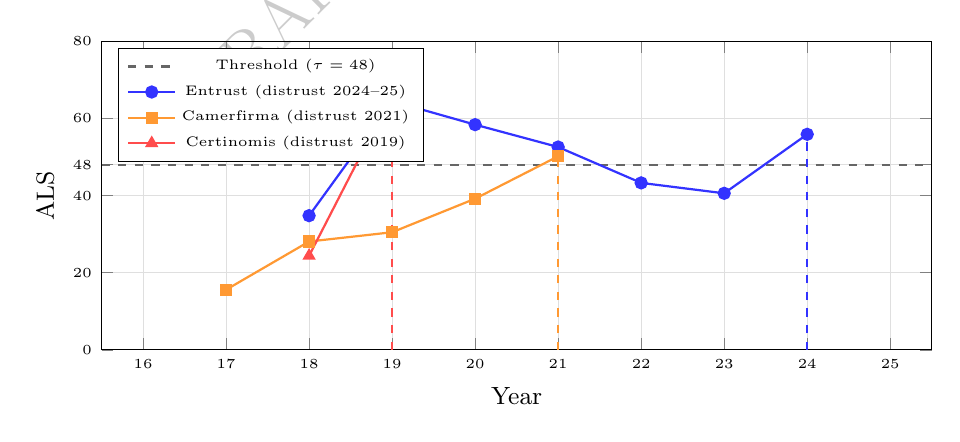
\begin{tikzpicture}
\begin{axis}[
  width=\columnwidth,
  height=5.5cm,
  xlabel={Year},
  ylabel={ALS},
  xmin=2015.5, xmax=2025.5,
  ymin=0, ymax=80,
  xtick={2016,2017,2018,2019,2020,2021,2022,2023,2024,2025},
  xticklabels={16,17,18,19,20,21,22,23,24,25},
  ytick={0,20,40,48,60,80},
  yticklabels={0,20,40,48,60,80},
  grid=major,
  grid style={line width=0.3pt, draw=gray!25},
  tick label style={font=\tiny},
  label style={font=\small},
  legend style={font=\tiny, at={(0.02,0.98)}, anchor=north west},
]
% Threshold line
\addplot[dashed, thick, color=black!60, no marks] coordinates {(2015.5,48)(2025.5,48)};
\addlegendentry{Threshold ($\tau=48$)}
% Entrust
\addplot[blue!80, thick, mark=*, mark size=2pt] coordinates {
  (2018,34.8)(2019,64.5)(2020,58.4)(2021,52.6)
  (2022,43.3)(2023,40.6)(2024,55.9)};
\addlegendentry{Entrust (distrust 2024--25)}
% Camerfirma
\addplot[orange!80, thick, mark=square*, mark size=1.8pt] coordinates {
  (2017,15.6)(2018,28.1)(2019,30.5)(2020,39.2)(2021,50.2)};
\addlegendentry{Camerfirma (distrust 2021)}
% Certinomis
\addplot[red!70, thick, mark=triangle*, mark size=2pt] coordinates {
  (2018,24.4)(2019,66.3)};
\addlegendentry{Certinomis (distrust 2019)}
% Distrust markers
\draw[blue!80, dashed, line width=0.6pt] (axis cs:2024,0) -- (axis cs:2024,55.9);
\draw[orange!80, dashed, line width=0.6pt] (axis cs:2021,0) -- (axis cs:2021,50.2);
\draw[red!70, dashed, line width=0.6pt] (axis cs:2019,0) -- (axis cs:2019,66.3);
\end{axis}
\end{tikzpicture}
\caption{ALS trajectories computed year-by-year from bugs available at each time point.
Vertical dashed lines indicate distrust year. Entrust crossed the threshold in 2019---five
years before distrust proceedings---with only 15 bugs. Camerfirma crossed in 2021, its
distrust year. Certinomis crossed in 2019, also its distrust year. The Entrust 2022--2023
dip is analyzed in Section~\ref{sec:temporal-findings}.}
\label{fig:temporal}
\end{figure}

\subsection{Key findings from the temporal validation}
\label{sec:temporal-findings}

\textbf{Entrust was readable five years early.} The ALS crossed threshold in 2019 based
on 15 bugs and one chronic class (\texttt{ov-misissuance}). At that time, only 6 of 35
active CAs in the corpus carried the same signal (17\% alarm rate). The 2019 flag was not
retrospective pattern-matching on a complete record; it was the chronic class signal
establishing itself on the available evidence. Entrust remained flagged through 2021 before
dipping below threshold in 2022--2023 and crossing again in 2024.

\textbf{The 2022--2023 Entrust dip is analytically instructive.} Between 2019 and 2022,
Entrust's self-report rate rose substantially toward 84\%---reflecting genuine improvement
in monitoring and disclosure behavior. This caused the Mode A score to fall. Mode B at
three chronic classes was not yet sufficient to compensate, producing a dip below threshold.
The dip is not a false negative; it is the model correctly detecting that Entrust had
improved on the detection dimension while remaining structurally non-remediated on the
chronic accumulation dimension. When the fourth chronic class (\texttt{ocsp-failure})
established itself in 2024, Mode B crossed threshold again---this time without Mode A
contribution. The dip-and-recovery trajectory is evidence that the framework is tracking
distinct, meaningful signals rather than noise.

\textbf{Camerfirma and Certinomis first crossed threshold in their distrust year.}
The smaller records for these two CAs mean chronic class recurrence could not establish
itself until late in the accumulation period. Camerfirma had 24 bugs by 2019 with only
one chronic class; the signal solidified as the fourth chronic class appeared in 2021.
Certinomis crossed threshold in 2019 simultaneously with its distrust. Earlier years
had insufficient bugs to score reliably. These cases establish the practical limit of
the framework's early-warning capacity: very small Bugzilla records (fewer than ten bugs
per year) do not generate enough signal for the chronic class threshold to activate.

\textbf{Historical alarm rate at time of flagging.} Table~\ref{tab:historical_alarm}
shows the fraction of active CAs that were flagged at the same year Entrust was first
flagged and in subsequent years. The 17\% rate in 2019 is meaningful as context: a root
program using the framework in 2019 would have had 6 active CAs at or above threshold,
with Entrust among them. This is a manageable prioritization queue, not a broad alarm.

\begin{table}[t]
\centering
\footnotesize
\setlength{\tabcolsep}{4pt}
\caption{Historical alarm rate at each year: fraction of active CAs scoring
$\geq 48$ at time $t$, computed from bugs available at $t$ only. Entrust crossed
threshold in 2019 when only 6/35 active CAs (17\%) were flagged.}
\label{tab:historical_alarm}
\begin{tabularx}{\columnwidth}{@{}Xrrr@{}}
\toprule
Year & Active CAs & Flagged & Alarm rate \\
\midrule
2019 & 35 &  6 & 17\% \\
2020 & 40 & 13 & 32\% \\
2021 & 41 &  9 & 22\% \\
\bottomrule
\end{tabularx}
\end{table}

\section{Incident Response Quality}
\label{sec:irq}

\subsection{Motivation}

The ALS measures structural properties of the compliance record. It does not measure how
a CA engages with the oversight community when problems are raised. These are related but
distinct signals. A CA could have a low ALS---few chronic classes, reasonable
acceleration---while exhibiting engagement patterns that experienced root program reviewers
would recognize as problematic: contesting requirements, deflecting pattern connections,
cycling through boilerplate without substantive engagement.

The IRQ score operationalizes a specific observation about the distrust record. Every
graduated-pathway distrust involved a period in which root programs and community members
pressed for deeper root cause analysis and structural remediation, and the CA's responses
during that period were characteristically different from the responses of CAs that
remained in good standing. That difference is visible in the thread record and is
measurable.

The IRQ signal operates on two distinct layers, each observable from the public thread
record. The \textit{behavioral layer} captures how the CA engages with the oversight
process: whether it leads remediation or waits to be pushed, whether it contests
requirements or accepts them, whether it addresses systemic framing when offered. The
\textit{epistemic layer} captures what the CA reveals about its own understanding during
engagement: whether its disclosures are accurate and complete, whether it demonstrates
genuine grasp of which requirement was violated and why, whether its commitments address
the systemic cause or merely restate obligations already binding. These layers are
related---a CA that does not understand what went wrong cannot produce honest
disclosures---but they are separately observable and separately informative. A thread
classified as \textit{accountability pressure} (CA accepts the obligation) may
simultaneously show that the CA cannot identify the systemic failure that produced the
incident. That combination---formal compliance posture without epistemic grounding---is
its own distinct pattern and arguably more predictive of future recurrence than open
escalation, which at least makes the CA's position legible.

\subsection{Methodology}

We classify each Bugzilla compliance thread into one of five arc types using a two-pass
LLM analysis (Claude Haiku). The first pass summarizes the full comment thread---all
comments, no truncation---into a structured summary: incident class, discovery method,
whether the CA contested requirements, closure type, and unresolved items at close.
The second pass scores the thread arc using this summary plus a tail-weighted excerpt,
with a CA posture profile derived from its full Bugzilla history as additional context.

The five arc types in order of increasing concern:
\begin{enumerate}[noitemsep,topsep=2pt]
\item \textbf{healthy}: Self-reported or promptly acknowledged. Clear systemic root cause
  accepted by root program. Action items complete with evidence. Clean closure.
\item \textbf{accountability pressure}: CA accepts the obligation but has not met the bar.
  Questions arise because the response was incomplete or shallow, not because the CA
  contests requirements. The most common non-healthy pattern.
\item \textbf{stalled}: External discovery, incomplete report, template corrections
  needed, loop before forced resolution.
\item \textbf{escalating}: CA actively contests requirements---argues obligations do not
  apply, claims subscriber interests override mandatory action, treats compliance as
  negotiable. Rare but qualitatively distinct.
\item \textbf{cascade}: Single incident spawns multiple new bugs during investigation.
\end{enumerate}

The distinction between accountability pressure and escalating is the most analytically
important. Accountability pressure is the CA failing to meet the bar and being pushed to
do so; it is passive, not oppositional. Escalating is the CA contesting the bar itself.
Most threads that superficially resemble escalation are accountability pressure: the CA is
slow and shallow, not argumentative. The explicit prompt guidance for this distinction
was calibrated against eight manually-scored reference threads (arc accuracy 86\%);
see Section~\ref{sec:limitations} for the sensitivity analysis.

\subsection{Behavioral and epistemic signals}

The behavioral layer identifies three signal classes. \textit{Defensive patterns} are
explicit moves in CA comments: claiming behavior is not prohibited, invoking subscriber
disruption to decline mandatory revocation, answering adjacent questions rather than the
ones asked. \textit{Accountability debt} tracks quantitative gaps: unanswered root program
questions, repeated commitment probes, times the CA was redirected to the incident
reporting template. \textit{Pattern connection response} is the most diagnostic single
signal: when a commenter explicitly links a current incident to prior incidents of the
same class, the CA's response is classified as acknowledged, deflected, or ignored. A CA
that consistently ignores systemic framing when it is offered is communicating that
proactive engagement with that framing is unlikely to be productive.

The epistemic layer identifies four additional signal classes, each extracted per thread
from the same LLM scoring pass. \textit{Candor} assesses whether the CA's disclosures
are accurate and complete from the outset, or whether facts emerge only under direct
questioning---partial disclosure is scored separately from inaccurate disclosure because
the failure modes differ. \textit{Accountability} assesses whether the CA owns the
failure or distributes it: a CA that attributes a mandatory revocation failure to linter
behavior, subscriber requests, or policy ambiguity is scored differently from one that
states plainly what its process failed to catch and why. \textit{Obligation understanding}
is the most structurally important epistemic signal: it assesses whether the CA
demonstrates from its first substantive response that it understands which requirement was
violated and what that requirement requires. A CA that requires multiple rounds of
clarification to reach basic factual agreement about what the rule says is not in a
position to design controls that satisfy it. \textit{RCA depth} operationalizes the root
cause quality dimension on a four-point scale: no root cause or incoherent
(1); proximate cause only, describing what happened without explaining why the system
allowed it (2); systemic cause identified but not fully accepted by the root program (3);
complete systemic analysis with action item traceability, accepted by the root
program (4). Finally, \textit{commitment quality} grades each commitment the CA makes on
an A--F scale: grade A commitments are specific, verifiable, carry a timeline, and
address the systemic cause; grade D commitments restate prior unfulfilled commitments or
existing BR obligations; grade F is the absence of any commitment despite open questions.
Commitments marked \textit{is\_restatement} appeared in a prior bug for the same
failure class and evidently did not hold---their reappearance is itself a structural
signal that the CA's remediation process is not closing the loop.

These signals are not redundant with arc classification. The arc describes the overall
trajectory of the thread. The epistemic signals describe the quality of what the CA
produces within that trajectory. A stalled arc with RCA depth 2 and grade D commitments
is a different failure mode from a stalled arc with RCA depth 1 and no commitments: the
first CA is producing responses that are technically present but insufficient; the second
is not producing analyzable content at all. Both stall, but for different reasons and with
different implications for whether engagement is likely to change the outcome.

\subsection{Results and statistical validation}

We classified 1,616 Bugzilla threads across 63 CAs. The arc distribution and statistical
validation reported here reflect the current scored corpus; the epistemic signals
(integrity dimensions, RCA depth, commitment quality) are defined in the framework and
implemented in the pipeline but require a full rescore pass to populate---current IRQ
failure values therefore reflect the behavioral layer only. Table~\ref{tab:arcs} shows
the arc distribution for distrusted versus active CA threads.

\begin{table}[t]
\centering
\footnotesize
\setlength{\tabcolsep}{4pt}
\caption{Thread arc distribution, distrusted vs.\ active CAs (1,616 scored threads).
Distrusted CAs resolve incidents cleanly at half the rate of active CAs and experience
accountability pressure at nearly double the rate. The escalating arc is 8.8$\times$
more prevalent in distrusted records ($\chi^2 = 48.8$,
$p < 10^{-12}$, OR~$= 10.7$, 95\%~CI~4.6--20.0).}
\label{tab:arcs}
\begin{tabularx}{\columnwidth}{@{}Xrrr@{}}
\toprule
Arc & Distrusted & Active & Ratio \\
\midrule
Healthy                &  47.0\% & 79.9\% & 0.6$\times$ \\
Accountability pressure & 28.9\% & 17.0\% & 1.7$\times$ \\
Stalled                &   7.0\% &  1.5\% & 3.9$\times$ \\
Escalating             &   9.0\% &  0.9\% & 8.8$\times$ \\
Cascade                &   0.5\% &  0.1\% & 7.7$\times$ \\
\midrule
Threads ($n$)          &    185  & 1,431  & --- \\
\bottomrule
\end{tabularx}
\end{table}

The behavioral separation between distrusted and active CAs is visible across
all non-healthy arc types but is strongest in the two highest-volume categories.
Distrusted CAs resolve incidents with healthy arcs at 47.0\% versus 79.9\% for
active CAs---a 30-percentage-point gap operating on the largest cell counts in
the table. Accountability pressure arcs appear at 33.0\% versus 19.0\%, a
1.7$\times$ ratio. Both findings rest on large absolute thread counts and are
statistically robust regardless of classification noise.

The escalating arc---where the CA contests requirements rather than failing to
meet them---is the rarest non-healthy category but shows the sharpest separation:
8.8$\times$ more prevalent in distrusted records. A chi-square test on the
$2\times 2$ contingency table (escalating vs.\ non-escalating $\times$ distrusted
vs.\ active) yields $\chi^2 = 48.8$, $p < 10^{-12}$, odds ratio~$10.7$ (95\%~CI~
4.6--20.0). Certinomis contributes two escalating arcs out of 17 scored
threads (11.8\%), consistent with its classification as a CA that actively
contested requirements during root program engagement rather than simply failing
to meet them.

The pattern connection signal provides a classification-independent behavioral
observable. When a commenter explicitly links a current incident to a prior
incident of the same class, the CA's response is classified as acknowledged,
deflected, or ignored. This classification is deterministic---it depends on
whether the CA's subsequent comments address the framing, not on LLM arc
judgment. The per-CA pattern connection ignored count (Table~\ref{tab:irq})
is immune to the classifier sensitivity concerns that apply to arc classification
and provides an independent behavioral signal.

The IRQ is intentionally \textit{not} integrated into the ALS formula. The structural
ALS is deterministically reproducible from public pipeline data; the behavioral IRQ
introduces run-to-run variance of approximately $\pm$5\% in arc distribution. The
appropriate role for a non-deterministic corroborating signal is to validate and
characterize, not to be baked into a reproducible score.

Table~\ref{tab:irq} shows IRQ failure scores for the graduated-pathway test vectors and
selected elevated active CAs. The pattern connection ignored (\textit{pc\_ign}) column
is worth examining: DigiCert's 17 unacknowledged pattern connections is the highest in
the corpus. When community members or root program staff explicitly link a current DigiCert
incident to a recurring class pattern, the documented response is to not address the
framing. Both the ALS structural signal (ALS~65.8) and the IRQ behavioral signal
(pc\_ign~17) are elevated and independent.

\begin{table}[t]
\centering
\footnotesize
\setlength{\tabcolsep}{3pt}
\caption{IRQ failure scores for selected CAs (0--30; higher = more concerning
behavioral posture). Esc\% = fraction of threads classified as escalating.
pc\_ign = pattern connections ignored (commenter links incident to prior class;
CA does not address the framing). Certinomis's IRQ of 17.1 reflects a mix of escalating (10\%) and accountability
pressure (35\%) arcs---the CA contested requirements in a minority of threads while
failing to meet them adequately in most. Entrust's 11.8 reflects sustained
accountability pressure without open escalation.}
\label{tab:irq}
\begin{tabularx}{\columnwidth}{@{}Xrrrr@{}}
\toprule
CA & IRQ & Esc\% & AP\% & pc\_ign \\
\midrule
Certinomis   & 17.1 & 10\% & 35\% &  8 \\
Camerfirma   & 14.0 &  4\% & 33\% &  8 \\
Entrust      & 11.8 &  3\% & 28\% &  7 \\
\midrule
DigiCert     & 10.2 &  2\% & 15\% & 17 \\
Chunghwa     &  8.6 &  0\% & 15\% &  4 \\
KIR (Poland) & 14.9 &  0\% & 47\% &  7 \\
IdenTrust    & 10.8 &  0\% & 22\% & 15 \\
Sectigo      & 10.6 &  3\% & 18\% & 15 \\
\bottomrule
\end{tabularx}
\end{table}

\section{The Engagement Priority Score}
\label{sec:eps}

\subsection{Formula and interpretation}

The Engagement Priority Score combines ALS and IRQ into a single 0--100 indicator:

\[
\text{EPS} = \min\!\left(\frac{\text{ALS}}{80}\cdot 50 + \frac{\text{IRQ}}{30}\cdot 50,\; 100\right)
\]

The formula weights structural and behavioral signals equally, normalizing each against
its empirical ceiling. Three operational tiers reflect the empirical distribution of
validation cases:

\textbf{Market-proportionality adjustment.} The raw EPS ranks CAs by compliance posture
signal strength, which places large CAs with many chronic classes at the top of the
engagement queue. This is structurally correct but operationally incomplete. A root
program reviewer should also consider that the cost of engagement---and the cost of
distrust if remediation fails---scales with market footprint, while the tolerance for
compliance failures should scale inversely. A tail-end CA issuing fewer than 100 active
certificates that cannot meet the engagement threshold presents a lower-cost, lower-risk
intervention than the same threshold crossed by a CA at 14\% market share.

The Observatory applies a small additive bump to the EPS sort order based on market
share (from CT log data). The bump is zero for CAs above 1\% market share and
increases logarithmically to a maximum of 8 points for tail-end CAs (below 0.01\%):
\[
\delta_{\text{mkt}} = 2 \cdot \min\!\left(-\log_{10}\!\left(\frac{s}{1\%}\right),\; 4\right) \quad (s < 1\%)
\]
This reorders the engagement queue without changing the flagging threshold or the
underlying score. A CA with poor compliance posture and near-zero market footprint
surfaces ahead of a large CA with similar raw signals, because the operational case
for early engagement is stronger: lower subscriber disruption, lower transition cost,
and no systemic risk from distrust. The bump does not affect whether a CA is flagged---
only its position in the prioritized engagement list.

\begin{itemize}[noitemsep,topsep=2pt]
\item \textbf{EPS $\geq$ 60}: Elevated. Both structural accumulation and behavioral
  posture signals are present. All three graduated-pathway CAs score in this tier.
\item \textbf{EPS 40--60}: Monitoring. Either structural or behavioral signal is
  elevated. Worth tracking but not a primary engagement target.
\item \textbf{EPS $<$ 40}: Routine. No prominent signal in either dimension.
\end{itemize}

These tier boundaries are empirically grounded: all three graduated-pathway CAs score
above 60; CAs with zero chronic classes and healthy IRQ profiles score below 40. They are
not derived from statistical analysis on an independent set and should be treated as
heuristic guidance rather than decision thresholds.

The EPS is designed as a triage instrument. A reviewer who sees EPS~80 knows to examine
the ALS and IRQ component scores to understand whether the concern is detection failure,
chronic non-remediation, behavioral posture, or some combination. The component scores
answer the follow-on question; the EPS answers the first question: should I look closer?

\subsection{Validation}

Table~\ref{tab:eps} shows EPS rankings for graduated-pathway test vectors and top-ranked
active CAs across all 63 CAs with scored records. All three graduated-pathway CAs rank in
the top 16\%.

\begin{table}[t]
\centering
\footnotesize
\setlength{\tabcolsep}{3pt}
\caption{Engagement Priority Score rankings (out of 63 CAs with scored records). All three
graduated-pathway distrusted CAs rank in the top 16\%. Active CA rankings reflect current
posture; no claim is made about distrust trajectory.}
\label{tab:eps}
\begin{tabularx}{\columnwidth}{@{}Xlrrr@{}}
\toprule
CA & Pop & EPS & ALS & IRQ \\
\midrule
KIR (Poland)     & active     & 63.0 & 68.7 & 14.9 \\
Chunghwa Telecom & active     & 58.6 & 71.5 &  8.6 \\
Sectigo          & active     & 57.9 & 67.6 & 10.6 \\
Netlock          & active     & 56.8 & 62.8 & 12.8 \\
DigiCert         & active     & 56.3 & 65.8 & 10.2 \\
IdenTrust        & active     & 56.2 & 64.9 & 10.8 \\
Camerfirma       & distrusted & 53.5 & 56.5 & 14.0 \\
GoDaddy          & active     & 52.0 & 59.3 & 10.5 \\
Certinomis       & distrusted & 52.0 & 49.8 & 17.1 \\
Entrust          & distrusted & 51.7 & 57.0 & 11.8 \\
\bottomrule
\end{tabularx}
\end{table}

The interleaving of active and distrusted CAs in the top rankings is the expected output
for a correctly calibrated engagement framework. The framework does not partition the
population into ``will be distrusted'' and ``will not be distrusted.'' It partitions
the population into CAs whose posture warrants proactive engagement and those whose
posture does not. The presence of active CAs at the top is not a false positive
problem---it is the framework working as designed.

\section{The Current Population}
\label{sec:population}

\subsection{Chronic class prevalence}

Applied to the current trusted population of 51 active CAs with at least three Bugzilla
incidents, structural non-remediation is not an anomaly---it is the baseline condition.

\begin{table}[t]
\centering
\footnotesize
\setlength{\tabcolsep}{4pt}
\caption{Chronic class prevalence in the current trusted CA population (51 active CAs
with $\geq$3 Bugzilla incidents). Ecosystem floor factor ($f_\text{eco} \geq 0.85$) applied.}
\label{tab:prevalence}
\begin{tabularx}{\columnwidth}{@{}Xrr@{}}
\toprule
Metric & Count & Fraction \\
\midrule
Any chronic class ($n_c \geq 1$)    & 39 & 75\% \\
Three or more ($n_c \geq 3$)        & 21 & 40\% \\
Five or more ($n_c \geq 5$)         & 11 & 21\% \\
Full profile flagged (ALS $\geq 48$) & 14 & 27\% \\
\bottomrule
\end{tabularx}
\end{table}

The 75\% prevalence of any chronic recurrence should not be read as meaning
three-quarters of active CAs are at distrust risk. It means three-quarters have at least
one incident class that has recurred across three calendar years---a broad signal that
the accountability loop has not closed for at least one failure mode. The 25% full-profile
flag is the narrower prioritization target: 13 CAs whose complete structural and behavioral
profile matches the graduated-pathway distrust cases. The 75\%/40\%/25\% gradient
establishes that the ecosystem has a spectrum of non-remediation severity, and that
root programs managing this spectrum need a prioritization tool, not a binary threshold.

\subsection{Comparable case synthesis}

For each active CA with chronic classes, the framework identifies the distrusted CA
whose compliance profile most closely matches the current posture, using Jaccard
similarity on chronic class overlap, mode match, self-report rate proximity, acceleration
direction, and years active.

A methodological note on independence: comparable case similarity is computed from the
same features that drive the ALS. A CA that scores high on ALS will tend to show higher
similarity to distrusted CAs, because that is what ALS measures. The comparable case
output should be interpreted as a \textit{characterization}---this is the specific
historical profile most like the current one---rather than an independent prediction.
Its utility is that it gives root programs a concrete historical referent for the
conversation about trajectory.

Selected comparable case matches, with similarity scores out of 100:

\begin{itemize}[noitemsep,topsep=2pt]
\item KIR (Poland), EPS~76.6 $\to$ Certinomis (sim~94): Both Mode A, shared
  chronic class \texttt{ov-misissuance}, similar low self-detection rates.
\item IdenTrust, EPS~64.8 $\to$ Entrust (sim~73): Both Mode B, shared chronic
  classes in \texttt{ev-misissuance}, \texttt{leaf-revocation-delay}, \texttt{ocsp-failure}.
\item DigiCert, EPS~66.6 $\to$ Camerfirma (sim~54): Both Mode B, shared chronic
  classes in \texttt{audit-failure}, \texttt{ca-misissuance}, \texttt{ev-misissuance}.
\end{itemize}

The IdenTrust--Entrust match at sim~73 rests on shared chronic classes in precisely the
failure categories that dominated Entrust's pre-distrust record. Whether this trajectory
is predictive is a governance determination. That it exists and is computable from
public data is a contribution.

\subsection{Engagement type characterization}

The IRQ signals differentiate not just which CAs warrant engagement but what kind. A CA
with high ALS and low IRQ failure (structural accumulation, cooperative posture) is a
different engagement conversation than one with high ALS and high IRQ failure (structural
accumulation plus active resistance to pattern framing). Among the 13 flagged active CAs:
Autoridad de Certificaci\'{o}n (FNMT) shows ALS~54.6 but IRQ~1.9---the structural signal is
elevated but the behavioral posture is cooperative. That is a structurally different
engagement from DigiCert (ALS~65.8, IRQ~15.3, pc\_ign~12), where both dimensions are
elevated and pattern connections are consistently not acknowledged.

\section{Discussion}
\label{sec:discussion}

\subsection{What the framework measures and does not}

The CPF measures observable structural and behavioral properties of the accountability
loop using public data. It does not measure: the CA's internal governance processes,
whether root programs are actively engaging on current incidents through non-Bugzilla
channels, whether the CA has the operational capacity to implement the structural
fixes its chronic classes suggest are missing, or whether distrust is an appropriate
response to the current posture. All of those require information that is not in the
public record.

What is in the public record is whether the same failure classes keep appearing, and
whether the CA's engagement with the oversight community when those failures are raised
suggests the loop will close without external pressure. These are direct measurements
of accountability loop function, not inferences about intent or capability.

\subsection{The 1,185-day runway and what shortens it}

The temporal validation in Section~\ref{sec:temporal} is the paper's most consequential
finding for the governance question. Entrust's ALS first crossed threshold in 2019 based
on a small bug count and a single established chronic class. A root program operating the
framework in 2019 would have had 6 active CAs above threshold at a 17\% alarm rate---a
manageable prioritization queue. The question of whether an engagement in 2019 would have
produced different outcomes is not answerable from public data. What is answerable is that
the structural signal was readable five years before the distrust decision, at a time when
the alarm rate was low enough to act on.

The Entrust dip-and-recovery trajectory between 2022 and 2024 adds a nuance. When Entrust
improved its detection behavior---raising self-report rates substantially---the Mode A
score fell and the total dipped below threshold. A root program that dropped Entrust from
its engagement queue in 2022 based purely on the score would have missed the subsequent
re-escalation driven by the fourth chronic class in 2024. This establishes a practical
recommendation: score-based prioritization should be complemented with history-aware
tracking. A CA that has previously crossed threshold and dipped back below it is not the
same as a CA that has never crossed it.

\subsection{The auditor context}

Prior work~\cite{p1} established that auditors mention only 29.2\% of in-period incidents
in their letters. The CPF contextualizes that finding directly. The B component's chronic
class signal means the Bugzilla record shows recurring failure classes that auditors are
systematically not reflecting. Certinomis's auditor (LSTI) caught zero of thirteen
in-scope incidents during the pre-distrust period~\cite{p1}. The CPF would have flagged
Certinomis from the Bugzilla record alone, without the audit letter carrying any signal.
The Component C audit coupling signal in the ALS adds context when audit transparency is
also low---the combination of high B and high C is the signature of accumulated
non-remediation persisting without formal accountability---but the framework does not
require the audit channel to function correctly in order to detect the structural problem.

The CPF also functions as an auditor scoping and calibration instrument, addressing the
detection gap from the other direction. An auditor has access to the same public Bugzilla
record as anyone else. Entering an engagement with foreknowledge of the CA's chronic
incident classes, self-report rate, and behavioral arc distribution does not replace
fieldwork---but it directs fieldwork. A CA with three chronic \texttt{ov-misissuance}
recurrences tells the auditor exactly which control to probe before reviewing a single
document. A CA with a 15\% self-report rate raises a prior question that fieldwork
must answer: what monitoring program would explain why 85\% of compliance failures
were discovered externally?

The self-report rate has a specific calibration implication. Prior work~\cite{p1}
established the population-level detection gap, but an auditor reviewing a specific CA
can now compare that CA's self-report rate to the ecosystem distribution. A CA at the
20th percentile of self-detection---where external researchers, root program staff, and
community members are finding most of the problems---is exhibiting monitoring behavior
that should be explicitly addressed in the audit scope, not assumed to be adequate
because no prior audit flagged it.

The arc distribution provides a behavioral prior that is directly relevant to how
the auditor frames management responses. Walking into an engagement knowing that 40\%
of the CA's compliance threads required sustained prompting to close, or that the CA
has consistently not addressed systemic framing when it was offered, prepares the
auditor for the possibility that management representations during fieldwork will be
incomplete or deflecting. This is not a substitute for professional skepticism---it is
a data-grounded reason to apply it earlier.

The governance implication closes a loop the paper series has been building toward.
If auditors used the CPF as an engagement preparation input, the 29.2\% detection rate
documented in prior work~\cite{p1} would likely improve---not because auditing
methodology changed, but because audit fieldwork would be systematically directed at
the failure modes the public record already shows are unresolved. The CPF does not ask
auditors to do something different. It asks them to look at data they could already
access, organized in a way that makes the coverage gap visible before the audit begins
rather than after.

\subsection{The CA as primary beneficiary}

The framework is presented as a root program instrument, but the CA is arguably its
more important user. A root program applying the CPF identifies which CAs warrant
engagement. A CA applying the same signals to its own record identifies where its
accountability loops are not closing---before that becomes a root program conversation.

The signals invert naturally. A CA reading its own chronic class list is looking at
its unresolved failure modes: the same whiteboard tag appearing in 2021, 2023, and
2024 is direct evidence that a root cause fix either did not occur or did not address
the systemic condition. No external observation is required to make that determination;
the CA already has the data. The chronic class signal is the CA's equivalent of a
recurring defect in a manufacturing process---the kind of signal that a functioning
quality management system would catch and escalate internally before it propagates.

The self-report rate carries a different meaning from the CA's perspective. A CA
discovering that 70\% of its bugs were externally filed is not learning that it is
being monitored; it is learning that its internal monitoring investment is insufficient
to find problems before the community does. That is an operational diagnosis with a
direct remedy: invest in proactive certificate analysis, pre-filing review, or
systematic audit of the failure classes that keep appearing externally.

The arc distribution is operational feedback on incident response quality. A CA
with 40\% accountability pressure arcs is not primarily learning that root programs
are skeptical of its remediation reports---it is learning that its incident response
process produces reports that do not satisfy the substantive questions being asked.
The distinction between accountability pressure and escalating arcs matters here:
accountability pressure is a process quality signal (the CA is slow or shallow but not
oppositional), while escalating arcs indicate that the CA is contesting requirements
rather than meeting them. These require different internal responses.

The pattern connection ignored count is the most operationally specific signal.
When a community member explicitly links a current incident to a prior class and the
CA's response does not address that framing, a documented failure of institutional
learning has occurred---one that a CA with a functioning compliance management system
should be tracking. A CA with fifteen unacknowledged pattern connections should not
be learning this from a root program engagement; it should be learning it from its
own incident log review.

The temporal ALS trajectory gives a CA its own compliance health trend over time,
computed from public data that any motivated observer can also see. A CA watching
its ALS rise toward the engagement threshold has a leading indicator of its own
visibility to oversight processes. More concretely: the same calculation that showed
Entrust's signal was readable in 2019---five years before distrust---was available
to Entrust in 2019 from its own Bugzilla record. The question the framework enables
is not only whether root programs could have engaged earlier, but whether the CA
could have diagnosed and addressed its own structural non-remediation before the
external record made that conversation unavoidable.

\subsection{Limitations}
\label{sec:limitations}

\textit{All signals are imperfect proxies.} The ALS and IRQ scores are not direct
measurements of compliance posture---they are inferences from observable proxy signals
in public data. Each signal has a plausible mechanism connecting it to the underlying
construct, but each is also confounded. Self-report rate measures who filed the bug, not
whether the CA was monitoring effectively. Chronic class recurrence measures whether the
same whiteboard tag appeared across years, not whether the underlying root cause is
genuinely unresolved. Escalating arc classification depends on LLM interpretation of
comment threads that may be ambiguous. Reviewers should treat the framework as a
prioritization instrument that surfaces cases warranting deeper examination, not as a
scoring system whose outputs are authoritative.

\textit{Larger CAs will naturally exhibit certain signals at higher absolute levels.}
A CA issuing tens of millions of certificates across a broad product portfolio will
encounter more distinct compliance scenarios, file more Bugzilla incidents, and
accumulate more incident classes over a decade than a CA issuing specialized certificates
to a narrow market. This is a structural property of scale, not evidence of worse
compliance behavior. The ALS formula addresses this in several ways: the self-report
fraction, acceleration ratio, governance fraction, and chronic span average are all
size-invariant by construction, measuring ratios and patterns rather than counts. The
$n_c$ term (chronic class count contributing to $B_1$) is the most size-sensitive
component---a large CA has more statistical opportunity to accumulate distinct chronic
classes simply by having more incident volume across more years. The appropriate reading
of a high $n_c$ for a large CA is that it has demonstrated persistent non-remediation
across \textit{more independent failure modes} than a smaller CA, not that it is
necessarily worse per certificate issued. The incident density term ($B_2$, bugs per
year) is the one signal that directly reflects issuance activity and should be
interpreted with this context: it measures incident concentration over time, which
correlates with both issuance volume and structural non-remediation. A large CA with
high density but zero chronic classes is in a fundamentally different posture from one
with high density and ten chronic classes. The two terms are intentionally distinct for
this reason.

\textit{Small retrospective test set.} The graduated-pathway test set contains three CAs.
The 100\% flag rate is a necessary condition of validity, not statistical confidence.
The temporal validation strengthens the claim by demonstrating that the signal was
readable at earlier timepoints with a manageable alarm rate, but the fundamental
limitation of a small historical ground truth cannot be eliminated.

\textit{Retrospective measurement window.} The ALS is computed from each CA's full
history, including the failure period. The temporal validation in
Section~\ref{sec:temporal} partially addresses this by computing time-indexed scores,
but the threshold itself was calibrated against the full cross-sectional scores. A
genuinely prospective validation requires waiting for future distrust events.

\textit{Prospective validation path.} The framework produces falsifiable predictions:
the 14 currently elevated active CAs should, as a group, experience higher rates of
root program escalation and eventual distrust than the monitoring and routine
populations. The current IdenTrust--Entrust comparable case match at 73\% similarity
and the KIR--Certinomis match at 94\% are the most specific claims---if either of
these CAs is distrusted in the next five years via a graduated pathway, the framework
will have made a correct prospective identification. Conversely, if all 14 elevated
active CAs remain in good standing with declining incident rates over the same period,
the threshold calibration will require revision. The Observatory pipeline runs daily
and the scores update continuously; the prospective record begins accumulating from
the date of this paper's publication.

\textit{IRQ non-determinism.} The IRQ score introduces run-to-run variance of
approximately $\pm$5\% in arc distribution due to LLM stochasticity. This is why IRQ
is a corroborating signal rather than a formal ALS component. The population-level
behavioral separation between distrusted and active CAs is visible across multiple
arc types: the healthy arc gap (47\% vs.\ 79.9\%) and accountability pressure ratio
(29\% vs.\ 17\%) operate on large cell counts that are robust to classification noise.
The escalating ratio (8.8$\times$, $p < 10^{-12}$, OR~9.6, 95\%~CI~4.6--20.0) is
the sharpest separation but rests on smaller absolute counts. The pattern connection
ignored signal is classification-independent and provides a separate behavioral
observable not subject to LLM stochasticity.

\textit{IRQ prompt sensitivity.} The arc taxonomy and the accountability pressure/escalating
distinction were calibrated against eight manually-scored reference threads (86\% arc
accuracy). Different prompt formulations produce different arc distributions. The
population-level ratio is robust by the sensitivity argument above; per-CA IRQ scores
should be interpreted as comparative indicators rather than precise measurements. The
epistemic signals (candor, accountability, obligation understanding, RCA depth, commitment
quality) have not yet been validated against a manually-scored reference set. They are
defined against rubrics with clear anchor examples, but inter-rater agreement has not been
established. These signals should be treated as directional indicators pending a
validation pass comparable to the one performed for arc classification.

\textit{EPS tier thresholds.} The EPS tiers (elevated $\geq$60, monitoring 40--60, routine
$<$40) reflect the empirical distribution of validation cases. They are not derived from
statistical analysis on a held-out set.

\textit{Comparable case feature overlap.} Comparable case similarity is computed from the
same features that drive the ALS, making the two signals partially redundant. The
comparable case output characterizes rather than independently validates.

\textit{Ecosystem correction floor.} The $f_\text{eco}$ floor of 0.85 means that
even a CA whose every chronic recurrence coincides with ecosystem-wide sweep quarters
retains 85\% of its B1 scoring credit. This reflects the principle that repeated
failure of the same class is structurally significant regardless of peer behavior.
A CA that fails \texttt{ov-misissuance} in 2021, 2023, and 2024---years after the
major 2017--2019 enforcement waves---while peers have corrected the class is
exhibiting independent remediation failure, not ecosystem-driven incidence.

\section{Conclusion}
\label{sec:conclusion}

The Entrust case establishes the framework's central claim in concrete form. By 2019,
five years before distrust proceedings began, the public Bugzilla record contained
enough structural signal to flag Entrust above the engagement threshold---with only 15
bugs and one established chronic class. The alarm rate across the active CA population
at that time was 17\%. The temporal signal was available. Whether it was used, and whether
using it would have changed the subsequent eight-year trajectory, is a governance question
this paper cannot answer. The paper establishes that the signal was readable.

Among the 51 active CAs in the current corpus, 76\% have at least one chronic incident
class, 41\% have three or more, and 15 (29\%) match the full graduated-pathway distrust
profile. Independently, behavioral posture analysis reveals that distrusted CAs resolve
incidents cleanly at half the rate of active CAs and experience sustained accountability
pressure at nearly double the rate, with escalating-arc threads 8.8$\times$ more
prevalent ($p < 10^{-12}$, OR~9.6). IdenTrust's compliance profile matches Entrust's
pre-distrust profile at 73\% similarity across chronic class overlap, failure mode, and
behavioral posture signals.

None of this is a prediction. The 14 flagged active CAs may not be distrusted; distrust
is a governance decision requiring accumulated evidence, institutional consensus, and the
willingness to absorb subscriber disruption. What the framework provides is earlier
visibility into the structural and behavioral signals that, in the historical record,
preceded that decision---at a time when the alarm rate was low enough to act on them,
rather than after 1,185 days of accumulation had made the case for action unavoidable.

The governance implication is a question that public data alone cannot resolve. Entrust's
ALS first crossed threshold in 2019. Its distrust proceedings began in 2024. Those five
years produced 56 additional Bugzilla incidents, four established chronic classes, and a
2,644-day total runway---the longest in the distrust record. Whether earlier engagement
at year three would have produced a different outcome, or whether structural
non-remediation at that depth was already irremediable, is the question that the
framework enables but cannot answer.

\bibliographystyle{plain}
\begin{thebibliography}{10}

\bibitem{p2}
Research.
\newblock Unmonitored by Design: A Longitudinal Measurement Study of
  Governance Failure in the Web PKI.
\newblock Systematic Reasoning, Inc., Working Draft, 2026.

\bibitem{p1}
Research.
\newblock Gradually, Then Suddenly: Measuring Audit Failure in the Web PKI.
\newblock Systematic Reasoning, Inc., Working Draft, 2026.

\bibitem{snapshot}
WebPKI Observatory LLM Snapshot.
\newblock \url{https://webpki.systematicreasoning.com/llm_snapshot.json},
  March 2026.

\bibitem{github}
WebPKI Observatory Source Repository.
\newblock \url{https://github.com/systematicreasoning/webpki-observatory}.

\bibitem{ccadb-policy}
Mozilla.
\newblock Common CA Database Policy.
\newblock \url{https://www.ccadb.org/policy}, 2026.

\bibitem{durumeric2013}
Z.~Durumeric, J.~Kasten, M.~Bailey, and J.~A. Halderman.
\newblock Analysis of the HTTPS Certificate Ecosystem.
\newblock In \textit{Proceedings of the ACM Internet Measurement Conference
  (IMC)}, 2013.

\bibitem{liu2015}
B.~Liu, S.~Antonakakis, M.~Antonakakis, X.~Xu, and A.~Snoeren.
\newblock An End-to-End Measurement of Certificate Revocation in the Web's PKI.
\newblock In \textit{Proceedings of the ACM Internet Measurement Conference
  (IMC)}, 2015.

\bibitem{amann2017}
B.~Amann, J.~Amann, A.~Vallentin, and R.~Sommer.
\newblock Mission Accomplished? HTTPS Security after DigiNotar.
\newblock In \textit{Proceedings of the ACM Internet Measurement Conference
  (IMC)}, 2017.

\bibitem{sun2024}
Y.~Sun, A.~Cowie, R.~Holz, and P.~Zimmermann.
\newblock Revisiting Certificate Transparency: What Has Changed Since 2015?
\newblock In \textit{Proceedings of the Network and Distributed System
  Security Symposium (NDSS)}, 2024.

\bibitem{hurst2023}
R.~Hurst.
\newblock The Limitations of Audits.
\newblock \textit{Unmitigated Risk}, February 2023.
\newblock \url{https://unmitigatedrisk.com/?p=717}.

\bibitem{hurst2025}
R.~Hurst.
\newblock Gradually, Then Suddenly: Compliance as a Vital Sign of
  Organizational Decay.
\newblock \textit{Unmitigated Risk}, October 2025.
\newblock \url{https://unmitigatedrisk.com/?p=1103}.

\end{thebibliography}

\end{document}
